% ch07a Local magnetic moments in metals, part a (书页 51-69 / 分册p001-019)
% 第7章 Local magnetic moments in metals
\chapter{金属中的局域磁矩}

Matthias 及其合作者在一系列针对非磁性金属——即没有永久磁矩的金属——的电子自旋共振（ESR）和核磁共振（NMR）实验中，在 ESR 线形里观察到了长寿命局域自旋包存在的惊人证据（M1960）。这些数据表明局域磁矩能够持续存在。人们很快查明，这一磁矩源于微量磁性杂质的存在。虽然研究过的体系多种多样——例如 Cu、Ag、Au 等主体材料中的 Mn、Fe 及其他铁族杂质——但所有杂质离子的共同特点是都拥有一个或多个空的内壳层轨道。此外，实验还表明，改变磁性杂质的种类和数量并不一定导致非磁性金属中局域磁矩的形成。这一发现更增添了问题的趣味，并确立了局域磁矩的形成这一问题在理解固体中磁性与输运方面的核心地位。本章中我们将描述局域磁矩的起源，重点放在安德森（Anderson）模型（A1961）上——该模型脱颖而出，成为金属中局域磁矩形成的标准微观图像。

\section{局域磁矩：唯象描述}

非磁性金属中的杂质可以产生局域磁矩，只要杂质上的某个电子态被单占据——至少在实验的时间尺度上如此。弗里德德尔（Friedel）（F1958）最先引入了一个唯象模型来解释局域磁矩的出现。在他的模型中，杂质的效果等效于产生一个势，该势实际上是一个深的库仑芯加上一个依赖于角动量的离心势垒 $\sim\ell(\ell+1)/r^{2}$，其中距离 $r$ 从杂质中心量起。这样的势可以支撑束缚态。远在费米能级之下的束缚态会被双占据，无需磁矩。然而，若相应于上、下自旋的能级并不简并，则在费米能级附近杂质势的束缚态或共振态中可以形成局域磁矩。

安德森（A1961）采纳弗里德德尔的基本思想，发展了一个局域磁矩形成的单带模型，其要点如下。非磁性金属主体（典型的如钛这样的过渡金属）中的能带用一组布洛赫态表示。把单粒子能量从费米海的顶部量起——这等价于取费米能 $\epsilon_{\mathrm{F}}=0$——我们取带能量为 $\epsilon_{\mathbf{k}}=\hbar^{2}k^{2}/2m-\hbar^{2}k_{\mathrm{F}}^{2}/2m$。杂质则被简单地处理为一个放置了单个电子轨道的局域格点。

\begin{table}[H]\centering
\caption*{表 7.1\quad 各种库仑矩阵元}\label{tab:auto:7.1}
\begin{tabular}{cllc}
\toprule
符号 & 积分 & 描述 & 量级\\
\midrule
$U$ & $\langle ii|V_{\mathrm{ee}}|ii\rangle$ & 在位 & $20\,\mathrm{eV}$\\
$V$ & $\langle ij|V_{\mathrm{ee}}|ij\rangle$ & 最近邻 & $2$--$3\,\mathrm{eV}$\\
$Y$ & $\langle ij|V_{\mathrm{ee}}|ji\rangle$ & 交换 & $1/40\,\mathrm{eV}$\\
\bottomrule
\end{tabular}
\end{table}

虽然这种简化没有反映 Co、Fe、Ni 等典型杂质 $d$ 轨道的五重简并，但这一缺陷并不关键。我们用 $\phi_{d}(\mathbf{r})$ 记该轨道的波函数。把一个自旋向上或向下的电子放到杂质上所需的能量是 $\epsilon_{d}$。该轨道既可以被单占据，也可以被两个自旋相反的电子占据。后一种情形付出的能量是 $U$，它物理上来自电子之间的库仑排斥，因而由下式给出：
\begin{equation*}
U=\langle dd|V_{\mathrm{ee}}|dd\rangle=\int\mathrm{d}\mathbf{r}_{1}\,\mathrm{d}\mathbf{r}_{2}\,|\phi_{d}(\mathbf{r}_{1})|^{2}\frac{e^{2}}{|\mathbf{r}_{1}-\mathbf{r}_{2}|}|\phi_{d}(\mathbf{r}_{2})|^{2}.\tag{7.1}
\end{equation*}

库仑排斥的效果是有利于杂质能级的单占据。安德森模型的最后一个要素是杂质能级与金属中能带的 $\mathbf{k}$ 态之间保持自旋的耦合，由矩阵元 $V_{\mathbf{k}d}$ 描述。这一相互作用导致带态与杂质能级的杂化。基本的安德森哈密顿量即为
\begin{equation*}
H^{\mathrm{A}}=\sum_{\mathbf{k}\sigma}\epsilon_{\mathbf{k}}a_{\mathbf{k}\sigma}^{\dagger}a_{\mathbf{k}\sigma}+\sum_{\sigma}\epsilon_{d}n_{d\sigma}+\sum_{\mathbf{k}\sigma}V_{\mathbf{k}d}\left(a_{\mathbf{k}\sigma}^{\dagger}a_{d\sigma}+a_{d\sigma}^{\dagger}a_{\mathbf{k}\sigma}\right)+Un_{d\uparrow}n_{d\downarrow},\tag{7.2}
\end{equation*}
其中 $a_{\mathbf{k}\sigma}^{\dagger}$ 在带态中产生电子，$a_{d\sigma}^{\dagger}$ 在杂质上产生一个自旋为 $\sigma$ 的电子，而 $n_{d\sigma}=a_{d\sigma}^{\dagger}a_{d\sigma}$ 是自旋为 $\sigma$ 的局域电子的粒子数算符。

安德森模型只包含两个局域电子之间的在位库仑排斥。此外，一个局域电子还会与其他格点上的局域电子相互作用。不过这些额外的项一般都很小。为估计这些附加相互作用的大小，哈伯德（Hubbard）（H1964）对过渡金属中的 $3d$ 电子假设了一个晶格模型，其中每个格点——记作 $i,j,\dotsc$——上放置一个局域态，并计算了如下形式的库仑势的一系列矩阵元：
\begin{equation*}
\langle i|\langle j|V_{\mathrm{ee}}|k\rangle|l\rangle=\int\mathrm{d}\mathbf{r}_{1}\,\mathrm{d}\mathbf{r}_{2}\,\phi_{i}^{*}(\mathbf{r}_{1})\phi_{j}^{*}(\mathbf{r}_{2})\frac{e^{2}}{|\mathbf{r}_{1}-\mathbf{r}_{2}|}\phi_{l}(\mathbf{r}_{2})\phi_{k}(\mathbf{r}_{1}).\tag{7.3}
\end{equation*}
各种库仑矩阵元的量级列于表 7.1。

在此表中 $i$ 与 $j$（$i\neq j$）表示最近邻格点。最近邻项是相邻格点上电子密度之间的直接库仑能，而“交换”项是对应的交换能，如第 5 章所讨论。可以看出，$U$ 是库仑相互作用中最大的贡献，因此在许多涉及强关联电子的固体问题中——例如哈伯德模型（H1964）——只保留 $U$ 项。一般而言，仅仅纳入 $U$ 并不保证所有相关物理都能得到描述。聚乙炔就是一个著名的例子（BC1989），其中 $V$ 以及其他库仑矩阵元在二聚化物理和光学性质中都起着关键作用。这里，额外的密度–键矩阵元 $X=\langle ii|V_{\mathrm{ee}}|ij\rangle$ 和键–键矩阵元 $\tilde{Y}=\langle ii|V_{\mathrm{ee}}|jj\rangle$——在过渡金属中量级分别为 $1/2\,\mathrm{eV}$ 和 $1/40\,\mathrm{eV}$——是重要的。“密度”一词指 $k=i$ 的情形，此时相应的波函数给出格点 $i$ 上的电子密度；“键”贡献得名于它们仅在电子在两个相邻局域态上有非零交叠时才不为零。

库仑相互作用有利于局域磁矩的形成，因为它倾向于抑制格点的双占据。另一方面，杂质能级与带态的强杂化在杂质上引起的电荷涨落则倾向于抹平局域磁矩。正如我们将看到的，衡量这一耦合的能量尺度，本质上是耦合导致初始处于杂质态的电子与带中某个 $\mathbf{k}$ 态之间发生跃迁（以及反向跃迁）的速率。由费米黄金定则，电子从杂质跃迁到金属能带中动量为 $\mathbf{k}$ 的态的速率为
\begin{equation*}
\frac{1}{\tau}=2\pi\frac{|V_{\mathbf{k}d}|^{2}N(\epsilon_{d})}{\hbar}\equiv\frac{2\Delta}{\hbar},\tag{7.4}
\end{equation*}
其中 $N(\epsilon_{d})$ 是在杂质能量 $\epsilon_{d}$ 处单一自旋的电子 $\mathbf{k}$ 态密度。作为这类虚跃迁的结果，杂质上的能级将被展宽；展宽的宽度由能量尺度 $\Delta$ 控制。我们把 $\Delta$ 称为杂化能，因为这个能量完全来自带态与杂质态之间的交叠。

安德森模型的物理由几个参量支配：杂质能量 $\epsilon_{d}$ 的大小及其相对于费米能级的位置、在位排斥能 $U$，以及杂化能 $\Delta$。作为示例，让我们考虑强杂化与弱杂化两个极限。在弱杂化情形 $U\gg\epsilon_{d}\gg\Delta$ 下，在杂质上双占据 $d$ 能级的代价远超 $\epsilon_{d}$ 和杂化能 $\Delta$。这一极限下系统一般支持局域磁矩的形成。我们一般假定杂质能级位于费米海之下，$\epsilon_{d}<0$。热平衡时，能量为 $\epsilon_{d}$ 的态至少被单占据。往杂质上放两个电子的代价是 $2\epsilon_{d}+U$。如果 $2\epsilon_{d}+U$ 超过费米能，即 $2\epsilon_{d}+U>0$，杂质的上能级不被占据，杂质是磁性的。这种情形的能级图示于图 7.1(a)。然而，在某些实验情形——例如 $\mathrm{SmB}_{6}$ 这样的稀土化合物和重费米子体系——杂质能级非常靠近费米能级。在这些“混价”情形中，杂化能的微小变化就会导致局域磁矩的消失。考虑 $U\gg\Delta\gg\epsilon_{d}$ 的情形，此时上能级仍远在费米能级之上，于是下杂质态的绝对能量小于该态的宽度。结果，这个态的占据数发生快速涨落，如图 7.1(b) 所示。这一区域是非磁性的。

接着考虑 $U$ 与 $\Delta$ 相比很小的区域。此时决定物理的是 $\Delta$ 而非 $U$。由于每个能级的展宽超过了双占据的能量代价，杂质被部分占据，一个自旋向上和一个自旋向下的电子以相等的概率占据。这个态不是磁性的，因为上、下自旋能级的占据相等。这种状态被称为局域自旋涨落（localized spin fluctuation）。通过调节 $U$ 和 $\Delta$，我们可以从磁性态连续地调到局域自旋涨落态；因此该模型是讨论局域磁矩形成物理的一个很好的出发点。

\begin{figure}[H]\centering
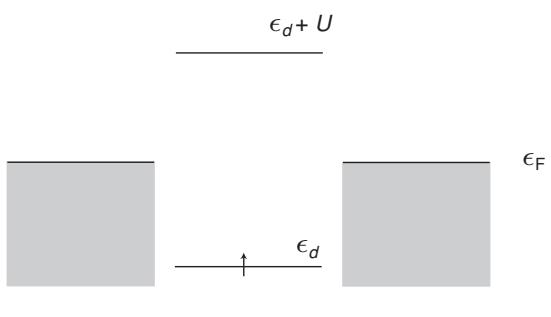
\includegraphics[width=0.6\textwidth]{figs/ch07/fig_7.1_a.jpg}\\[2pt]
{\small (a)}\\[12pt]
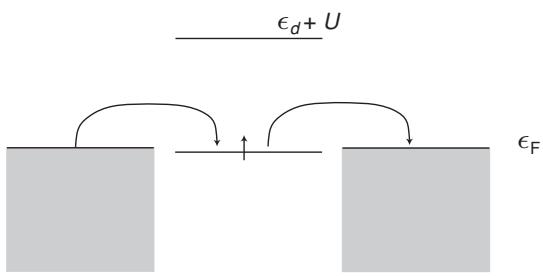
\includegraphics[width=0.6\textwidth]{figs/ch07/fig_7.1_b.jpg}\\[2pt]
{\small (b)}
\caption*{图 7.1\quad 局域弱耦合区域 $U\gg\Delta$（$\Delta$ 为杂化能）下安德森模型的能级图。左右两块阴影区画的是主体金属能带中同样的电子态——在这个问题中习惯这样画，以强调从连续带到局域态再到连续带的虚二阶跃迁。费米能级固定在 $\epsilon_{\mathrm{F}}=0$。杂质上可用的单粒子态能量，在能级未被占据时为 $\epsilon_{d}$，在能级已被单占据时为 $\epsilon_{d}+U$。(a) 当 $\epsilon_{d}$ 足够低于费米面时，有利于局域磁矩的形成。(b) 混价区域 $U\gg\Delta\gg\epsilon_{d}$ 下的能级图。下杂质能级非常接近费米面。杂质上的电荷涨落很快，导致杂质上的局域自旋涨落。这种情形不是磁性的。}\label{fig:auto:7.1}
\end{figure}

\section{杂质态密度}

理解局域磁矩形成所需的核心量是杂质各态的占据。如果这些态被某一给定自旋的电子占据的概率大于被另一自旋占据的概率，该格点就会带有局域磁矩。杂质格点的占据由如下计算得到：系统中某个已被占据的能量本征态上的电子被发现处于杂质上的概率。若 $\langle n|$ 是局域磁矩哈密顿量 $H^{\mathrm{A}}$ 的能量为 $\epsilon_{n\sigma}$ 的本征态，则 $|\langle n\sigma|d\sigma\rangle|^{2}$ 就是态 $|n\sigma\rangle$ 与杂质格点 $|d\sigma\rangle$ 交叠的概率。由于杂化耦合 $V_{\mathbf{k}d}$，这一交叠不为零。自旋为 $\sigma$ 的电子在杂质上的净占据，由对所有能量 $\epsilon\leq\epsilon_{\mathrm{F}}$ 的被占据电子态求和给出：
\begin{equation*}
\langle n_{d\sigma}\rangle=\sum_{n,\epsilon_{n\sigma}\leq\epsilon_{\mathrm{F}}}|\langle n\sigma|d\sigma\rangle|^{2}=\int_{-\infty}^{\epsilon_{\mathrm{F}}}\mathrm{d}\epsilon\,\rho_{d\sigma}(\epsilon),\tag{7.5}
\end{equation*}
其中杂质上的态密度为
\begin{equation*}
\rho_{d\sigma}(\epsilon)=\sum_{n}\delta(\epsilon_{n\sigma}-\epsilon)|\langle n\sigma|d\sigma\rangle|^{2}.\tag{7.6}
\end{equation*}
局域磁矩形成的判据是 $\langle n_{d\sigma}\rangle\neq\langle n_{d-\sigma}\rangle$。

杂质上的相互作用项使得构造单粒子能级和杂质态密度变得不再平庸。为解决这一问题，我们对这个相互作用问题采用平均场或哈特里–福克近似，在此近似下单粒子能级有良好的定义。由这一步骤得到的局域磁矩形成判据，在预言磁性合金中局域磁矩的出现方面实际上取得了巨大的成功（GZ1974）。在哈特里–福克近似下，系统基态具有形式
\begin{equation*}
|\Phi_{0}\rangle=\prod_{\epsilon_{n}<\epsilon_{\mathrm{F}}}a_{n\sigma}^{\dagger}|0\rangle,\tag{7.7}
\end{equation*}
其中
\begin{equation*}
a_{n\sigma}^{\dagger}=\sum_{\mathbf{k}}\langle\mathbf{k}\sigma|n\sigma\rangle a_{\mathbf{k}\sigma}^{\dagger}+\langle d\sigma|n\sigma\rangle a_{d\sigma}^{\dagger}\tag{7.8}
\end{equation*}
是带态与杂质态的线性组合。用新态（式 (7.8)）表示的哈特里–福克近似下，单体哈密顿量为
\begin{equation*}
H_{\mathrm{HF}}^{\mathrm{A}}=\sum_{n\sigma}\epsilon_{n\sigma}a_{n\sigma}^{\dagger}a_{n\sigma}.\tag{7.9}
\end{equation*}

对哈密顿量作哈特里–福克近似，相当于把相互作用项 $Un_{d\uparrow}n_{d\downarrow}$ 替换为 $U\langle n_{d\uparrow}\rangle n_{d\downarrow}+U\langle n_{d\downarrow}\rangle n_{d\uparrow}-U\langle n_{d\uparrow}\rangle\langle n_{d\downarrow}\rangle$，其中平均在态 $|\Phi_{0}\rangle$ 中取。最后一项只是把能量零点整体平移；因为它不影响局域磁矩的物理，我们把它丢掉。把缺陷格点能量重新定义为
\begin{equation*}
E_{d\sigma}=\epsilon_{d}+U\langle n_{d-\sigma}\rangle,\tag{7.10}
\end{equation*}
之后，安德森哈密顿量的哈特里–福克近似即为
\begin{equation*}
H_{\mathrm{HF}}^{\mathrm{A}}=\sum_{\sigma}E_{d\sigma}n_{d\sigma}+\sum_{\mathbf{k}\sigma}\epsilon_{\mathbf{k}}n_{\mathbf{k}\sigma}+\sum_{\mathbf{k}\sigma}V_{\mathbf{k}d}\left(a_{\mathbf{k}\sigma}^{\dagger}a_{d\sigma}+a_{d\sigma}^{\dagger}a_{\mathbf{k}\sigma}\right).\tag{7.11}
\end{equation*}
可以看到，对带在位库仑排斥的哈密顿量作哈特里–福克近似，不过是对格点能量作一个简单的重正化；量 $E_{d\sigma}$ 在局域磁矩形成的平均场理论中扮演关键角色。局域磁矩的判据 $\langle n_{d\sigma}\rangle\neq\langle n_{d-\sigma}\rangle$ 等价于条件 $E_{d\sigma}\neq E_{d-\sigma}$。一旦定义了单粒子能级，就容易证明式 (7.9) 与 (7.11) 等价（习题 7.3）。

单粒子能量 $\epsilon_{n\sigma}$ 通过算符运动方程定义：
\begin{equation*}
\left[H_{\mathrm{HF}}^{\mathrm{A}},a_{n\sigma}^{\dagger}\right]=\epsilon_{n\sigma}a_{n\sigma}^{\dagger}.\tag{7.12}
\end{equation*}
为计算式 (7.12) 中的对易子，我们利用对易关系
\begin{equation*}
\begin{aligned}
\left[H_{\mathrm{HF}}^{\mathrm{A}},a_{\mathbf{k}\sigma}^{\dagger}\right]&=\sum_{\mathbf{k}'\sigma}\epsilon_{\mathbf{k}'}\left[a_{\mathbf{k}'\sigma}^{\dagger}a_{\mathbf{k}'\sigma},a_{\mathbf{k}\sigma}^{\dagger}\right]+\sum_{\mathbf{k}'\sigma}V_{\mathbf{k}'d}\left[\left(a_{\mathbf{k}'\sigma}^{\dagger}a_{d\sigma}+a_{d\sigma}^{\dagger}a_{\mathbf{k}'\sigma}\right),a_{\mathbf{k}\sigma}^{\dagger}\right]\\
&=\epsilon_{\mathbf{k}}a_{\mathbf{k}\sigma}^{\dagger}+V_{\mathbf{k}d}a_{d\sigma}^{\dagger}
\end{aligned}\tag{7.13}
\end{equation*}
和
\begin{equation*}
\left[H_{\mathrm{HF}}^{\mathrm{A}},a_{d\sigma}^{\dagger}\right]=E_{d\sigma}a_{d\sigma}^{\dagger}+\sum_{\mathbf{k}}V_{\mathbf{k}d}a_{\mathbf{k}\sigma}^{\dagger},\tag{7.14}
\end{equation*}
并得到
\begin{equation*}
\begin{aligned}
\left[H_{\mathrm{HF}}^{\mathrm{A}},a_{n\sigma}^{\dagger}\right]&=\sum_{\mathbf{k}}\langle\mathbf{k}\sigma|n\sigma\rangle\left(\epsilon_{\mathbf{k}}a_{\mathbf{k}\sigma}^{\dagger}+V_{\mathbf{k}d}a_{d\sigma}^{\dagger}\right)+\langle d\sigma|n\sigma\rangle\left(E_{d\sigma}a_{d\sigma}^{\dagger}+\sum_{\mathbf{k}}V_{\mathbf{k}d}a_{\mathbf{k}\sigma}^{\dagger}\right)\\
&=\epsilon_{n\sigma}\sum_{\mathbf{k}}\langle\mathbf{k}\sigma|n\sigma\rangle a_{\mathbf{k}\sigma}^{\dagger}+\langle d\sigma|n\sigma\rangle a_{d\sigma}^{\dagger}.
\end{aligned}\tag{7.15}
\end{equation*}
于是
\begin{equation*}
\epsilon_{n\sigma}\langle\mathbf{k}\sigma|n\sigma\rangle=\epsilon_{\mathbf{k}}\langle n\sigma|\mathbf{k}\sigma\rangle+V_{\mathbf{k}d}\langle d\sigma|n\sigma\rangle\tag{7.16}
\end{equation*}
以及
\begin{equation*}
\epsilon_{n\sigma}\langle n\sigma|d\sigma\rangle=E_{d\sigma}\langle d\sigma|n\sigma\rangle+\sum_{\mathbf{k}}\langle\mathbf{k}\sigma|n\sigma\rangle V_{\mathbf{k}d}.\tag{7.17}
\end{equation*}
式 (7.16) 与 (7.17) 定义了单粒子能级 $\epsilon_{n\sigma}$。显式解留作课后练习（习题 7.2），它需要从式 (7.16) 和 (7.17) 中消去态 $\langle n\sigma|d\sigma\rangle$ 与 $\langle n\sigma|\mathbf{k}\sigma\rangle$。

\subsection{杂质态密度}

既然我们已经说明了如何求出决定态密度的单粒子能级，现在就把这个量显式地算出来。我们将借助预解核（resolvent）即格林函数来进行计算，它使我们能够直接把杂质能级的宽度包括进来。我们首先改写态密度，利用关系
\begin{equation*}
\begin{aligned}
\delta(\epsilon-\epsilon_{n\sigma})&=\frac{1}{\pi}\lim_{\Gamma\to 0}\frac{\Gamma}{(\epsilon-\epsilon_{n\sigma})^{2}+\Gamma^{2}}\\
&=\frac{1}{2\pi\mathrm{i}}\lim_{\Gamma\to 0}\left[\frac{1}{\epsilon-\epsilon_{n\sigma}-\mathrm{i}\Gamma}-\frac{1}{\epsilon-\epsilon_{n\sigma}+\mathrm{i}\Gamma}\right]\\
&=-\frac{1}{\pi}\lim_{\Gamma\to 0}\mathrm{Im}\,\frac{1}{\epsilon-\epsilon_{n\sigma}+\mathrm{i}\Gamma}.
\end{aligned}\tag{7.18}
\end{equation*}
于是
\begin{equation*}
\rho_{d\sigma}(\epsilon)=-\frac{1}{\pi}\lim_{\Gamma\to 0}\mathrm{Im}\sum_{n}\frac{|\langle n\sigma|d\sigma\rangle|^{2}}{\epsilon-\epsilon_{n\sigma}+\mathrm{i}\Gamma}.\tag{7.19}
\end{equation*}
量 $(\epsilon-\epsilon_{n\sigma}+\mathrm{i}\Gamma)^{-1}$ 是与这个问题的格林函数相关的一个预解核。我们通过
\begin{equation*}
(E+\mathrm{i}\Gamma-H)G=1.\tag{7.20}
\end{equation*}
定义格林（算符）函数 $G(E+\mathrm{i}\Gamma)$。把 (7.20) 两边除以 $(E-H+\mathrm{i}\Gamma)$，并在 $H^{\mathrm{A}}$ 的一组完备本征态中展开，得到
\begin{equation*}
G(E+\mathrm{i}\Gamma)=\sum_{n}\frac{|n\rangle\langle n|}{E+\mathrm{i}\Gamma-E_{n}}\tag{7.21}
\end{equation*}
作为格林函数的谱分解，其中 $H|n\rangle=E_{n}|n\rangle$，且 $G$ 在本征能量 $E_{n}$ 处奇异、带有极点。$G$ 的本征函数便是 $|n\rangle$。

对单粒子哈密顿量 $H=H_{\mathrm{HF}}^{\mathrm{A}}$，我们通过
\begin{equation*}
\sum_{\beta}(E+\mathrm{i}\Gamma-H)_{\alpha\beta}G_{\beta\mu}=\delta_{\alpha\mu},\tag{7.22}
\end{equation*}
定义 $G$ 的矩阵元，其中下标 $\alpha$、$\beta$ 和 $\mu$ 标记带特定自旋的带态或杂质态，即分别为 $|\mathbf{k}\sigma\rangle$ 与 $|d\sigma\rangle$。由 $G$ 的定义及式 (7.19)，若 $G$ 用 $H$ 的精确本征态表示，就可以把 $\rho_{d\sigma}(\epsilon)$ 改写为
\begin{equation*}
\begin{aligned}
\rho_{d\sigma}&=-\frac{1}{\pi}\lim_{\Gamma\to 0}\mathrm{Im}\sum_{n}\frac{|\langle n\sigma|d\sigma\rangle|^{2}}{\epsilon-\epsilon_{n\sigma}+\mathrm{i}\Gamma}\\
&=-\frac{1}{\pi}\lim_{\Gamma\to 0}\mathrm{Im}\,\langle d\sigma|G(\epsilon+\mathrm{i}\Gamma)|d\sigma\rangle\\
&=-\frac{1}{\pi}\lim_{\Gamma\to 0}\mathrm{Im}\,G_{dd}^{\sigma}
\end{aligned}\tag{7.23}
\end{equation*}
式 (7.23) 把态密度与 $G$ 的对角矩阵元联系起来，是我们表述局域磁矩问题所需的主要关系。从格林函数与简化后哈密顿量的方程出发，对 $\alpha=\mu=d\sigma$ 我们得到
\begin{equation*}
(\epsilon+\mathrm{i}\Gamma-E_{d\sigma})G_{dd}^{\sigma}-\sum_{\mathbf{k}}V_{d\mathbf{k}}G_{\mathbf{k}d}^{\sigma}=1,\tag{7.24}
\end{equation*}
对 $\alpha=k\sigma$、$\mu=d\sigma$ 得到
\begin{equation*}
(\epsilon+\mathrm{i}\Gamma-\epsilon_{\mathbf{k}})G_{\mathbf{k}d}^{\sigma}-V_{\mathbf{k}d}G_{dd}^{\sigma}=0.\tag{7.25}
\end{equation*}
如果利用式 (7.25) 从式 (7.24) 中消去 $G_{d\mathbf{k}}^{\sigma}$，就得到
\begin{equation*}
G_{dd}^{\sigma}(\epsilon+\mathrm{i}\Gamma)=\left[\epsilon+\mathrm{i}\Gamma-E_{d\sigma}-\sum_{\mathbf{k}}\frac{|V_{\mathbf{k}d}|^{2}}{\epsilon+\mathrm{i}\Gamma-\epsilon_{\mathbf{k}}}\right]^{-1}.\tag{7.26}
\end{equation*}
（注：分母的零点正落在二阶微扰的布里渊–维格纳（Brillouin–Wigner）理论所算得的能量处，能量分母中保留了完整的 $\epsilon$。）若式 (7.26) 分母中没有最后一项，$G_{dd}^{\sigma}$ 的奇点便位于重正化后的格点能量 $E_{d\sigma}$ 处。

转移积分（transfer integral）$V_{\mathbf{k}d}$ 使杂质能级展宽。为看清这一展宽，我们把 $(G_{dd}^{\sigma})^{-1}$ 的最后一项改写为
\begin{equation*}
\sum_{\mathbf{k}}\frac{|V_{\mathbf{k}d}|^{2}}{\epsilon-\epsilon_{\mathbf{k}}+\mathrm{i}\Gamma}=\sum_{\mathbf{k}}|V_{\mathbf{k}d}|^{2}\frac{\epsilon-\epsilon_{\mathbf{k}}-\mathrm{i}\Gamma}{(\epsilon-\epsilon_{\mathbf{k}})^{2}+\Gamma^{2}}.\tag{7.27}
\end{equation*}
在 $\Gamma\to 0$ 的极限下，式 (7.27) 化为
\begin{equation*}
\begin{aligned}
\lim_{\Gamma\to 0}\sum_{\mathbf{k}}\frac{|V_{\mathbf{k}d}|^{2}}{\epsilon-\epsilon_{\mathbf{k}}+\mathrm{i}\Gamma}&=\mathrm{P}\left(\sum_{\mathbf{k}}\frac{|V_{\mathbf{k}d}|^{2}}{\epsilon-\epsilon_{\mathbf{k}}}\right)-\mathrm{i}\pi\sum_{\mathbf{k}}|V_{\mathbf{k}d}|^{2}\delta(\epsilon-\epsilon_{\mathbf{k}})\\
&=\mathrm{P}\left(\sum_{\mathbf{k}}\frac{|V_{\mathbf{k}d}|^{2}}{\epsilon-\epsilon_{\mathbf{k}}}\right)-\mathrm{i}\pi\langle|V_{\mathbf{k}d}|^{2}\rangle N(\epsilon),
\end{aligned}\tag{7.28}
\end{equation*}
其中 $\mathrm{P}$ 表示主值；我们用式 (7.18) 得到最终结果，并把 $|V_{\mathbf{k}d}|^{2}$ 换成其平均值 $\langle|V_{\mathbf{k}d}|^{2}\rangle$。式 (7.27) 的第一项是纯实的，因而表示 $d$ 杂质能级的一个移动。这一项只有当它作为能量的函数剧烈涨落时才影响物理。然而，主体能带的态密度 $N(\epsilon)$ 在 $E_{d\sigma}$ 变化的尺度上相当恒定。因此 (7.27) 的实部可以忽略，$G$ 变为
\begin{equation*}
G_{dd}^{\sigma}(\epsilon+\mathrm{i}\Gamma)=\frac{1}{\epsilon+\mathrm{i}\Gamma-E_{d\sigma}+\mathrm{i}\Delta},\tag{7.29}
\end{equation*}
其中 $2\Delta=2\pi\langle|V_{\mathbf{k}d}|^{2}\rangle N(\epsilon)$ 是杂质与传导电子之间的有效跃迁速率。

如果把 $E_{d\sigma}-\mathrm{i}\Delta$ 解释为新的格点能量，那么正如前面所言，$2\hbar/\Delta$ 就是杂质能级的寿命。由式 (7.23) 与 (7.29)，我们发现 $d$ 杂质处的态密度化为洛伦兹形式
\begin{equation*}
\rho_{d\sigma}(\epsilon)=\frac{1}{\pi}\frac{\Delta}{(\epsilon-E_{d\sigma})^{2}+\Delta^{2}}\tag{7.30}
\end{equation*}
正如所料，$\Delta$ 在其中表现为 $d$ 能级的半宽度。

\begin{figure}[H]\centering
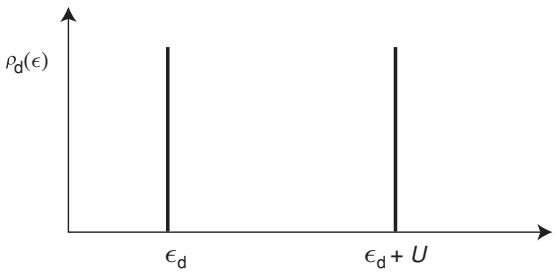
\includegraphics[width=0.6\textwidth]{figs/ch07/fig_7.2_a.jpg}\\[2pt]
{\small (a)}\\[12pt]
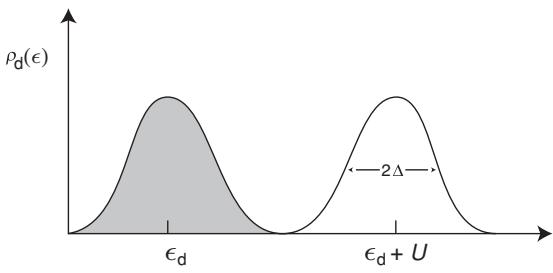
\includegraphics[width=0.6\textwidth]{figs/ch07/fig_7.2_b.jpg}\\[2pt]
{\small (b)}
\caption*{图 7.2\quad (a) 安德森模型中 $d$ 能级与 $\mathbf{k}$ 态之间的杂化为零时的单粒子态密度。单粒子能量 $\epsilon_{d}$ 处的尖峰对应杂质能级空着的情形，而 $\epsilon_{d}+U$ 处的尖峰对应杂质能级已被一个自旋相反的电子单占据的情形。在哈特里–福克层次上计入相互作用会把这两个峰移到 $E_{d\sigma}=\epsilon_{d}+U\langle n_{d-\sigma}\rangle$。(b) $d$ 态与 $\mathbf{k}$ 态混合时的态密度。每个态的宽度因杂化而展宽。与 (a) 一样，下面的能级对应杂质能级空着的情形，上面的峰对应一个给定自旋的电子已处于下面能级的情形。当下能级被占据而上能级空着时——如两峰下不相等的阴影所示——系统具有局域磁矩。}\label{fig:auto:7.2}
\end{figure}

当 $d$ 能级与传导态之间的杂化趋于零时，态密度趋于一个 $\delta$ 函数。为什么如此？态密度由格林函数的虚部决定。若当 $E$ 趋于实轴时 $G(E)$ 为纯实数，则 $G(E)$ 的奇点是能量上相距很远的单极点。此时态密度对应于在本征能量 $E_{d\sigma}=\epsilon_{d}+U\langle n_{d-\sigma}\rangle$ 处的一系列尖锐的（$\delta$ 函数型）峰。对于能级被一个给定自旋的电子单占据的情形，两个极点被在位库仑排斥 $U$ 分开，如图 7.2(a) 所示。只要 $d$ 能级与导带中的 $\mathbf{k}$ 态之间没有混合，这种状况就保持不变。一旦开启混合，极点便离开实轴，使纯粹的 $d$ 能级展宽。所得能谱在能量上不再分得很开（见图 7.2(b)）。

\section{格林函数}

这里有必要离题谈一谈格林函数。首先，我们称之为格林函数（Green functions）而不是“格林的函数”（Green's functions）——后者不合语法。试看同样不合语法的构造“贝塞尔的函数”（the Bessel's function），没有人这样用。尽管如此，我们仍会使用“格林定理”（Green's theorem）的说法，因为那毕竟是格林本人的定理。

把式 (7.20) 求逆，得到 $G=(E-H+\mathrm{i}\Gamma)^{-1}$，因而 $G$ 是哈密顿量希尔伯特空间中的一个算符。这使我们可以对它作谱分解，即用哈密顿量的本征态 $H|n\rangle=E_{n}|n\rangle$ 表示为
\begin{equation*}
G=\sum_{n}\frac{|n\rangle\langle n|}{E-E_{n}+\mathrm{i}\Gamma},\tag{7.31}
\end{equation*}
这里 $\Gamma$ 是一个正常数，它把 $G$ 的极点抬离实轴、移到紧靠实轴的下方。于是 $G$ 在上半平面解析。因此，其傅里叶变换
\begin{equation*}
G_{nn}=\int\frac{\mathrm{d}E}{2\pi}\langle n|G|n\rangle\mathrm{e}^{-\mathrm{i}Et/\hbar}=\frac{1}{2\pi}\int\mathrm{d}E\,\frac{\mathrm{e}^{-\mathrm{i}tE/\hbar}}{E-E_{n}+\mathrm{i}\Gamma},\tag{7.32}
\end{equation*}
只有在围道于下半平面闭合时才不为零。这直接导致 $G$ 的因果性。若 $t<0$，这个积分必须通过在上半平面闭合围道来收尾，才能给出有限结果。由于 $G$ 在那里解析，我们发现 $t<0$ 时 $G=0$。而当 $t>0$ 时，我们可以在下半平面闭合围道、包住极点，得到有限结果
\begin{equation*}
G_{nn}=-\mathrm{i}\,\mathrm{e}^{-\mathrm{i}E_{n}t/\hbar},\quad t>0.\tag{7.33}
\end{equation*}
极限 $\Gamma=0$ 是在算完围道之后取的。这种二分的时间行为表明 $G$ 是因果函数。对自由粒子这一简单情形，$E_{n}=p^{2}/2m$，格林函数化为
\begin{equation*}
G(p,E)=\frac{1}{E-p^{2}/2m+\mathrm{i}\Gamma}.\tag{7.34}
\end{equation*}

\subsection{格林函数：一般定义}

格林函数有着悠久的历史。它的正式定义是带单位间断（空间与时间上均有）的齐次微分方程的一般解
\begin{equation*}
\left(-\mathrm{i}\hbar\partial_{t}+H\right)G(\mathbf{r},t;\mathbf{r}',t')=-\hbar\delta(\mathbf{r}-\mathbf{r}')\delta(t-t'),\tag{7.35}
\end{equation*}
右端清楚地表明，无论 $G$ 是什么，它都保持时间和空间平移不变性。考虑傅里叶变换
\begin{equation*}
G(\mathbf{r},t;\mathbf{r}',t')=\int_{-\infty}^{\infty}G(\mathbf{r},\mathbf{r}';\varepsilon)\,\mathrm{e}^{-\mathrm{i}\varepsilon(t-t')/\hbar}\frac{\mathrm{d}\varepsilon}{2\pi}.\tag{7.36}
\end{equation*}
这个定义中隐含 $\varepsilon$ 上减去了一个虚部，即 $\varepsilon\to\varepsilon+\mathrm{i}\Gamma$。当 $t>t'$ 时我们得到有限结果；在相反区域，即 $t<t'$ 时，$G=0$。具有这种因果响应的格林函数称为推迟格林函数（retarded Green function）。

我们用费米型场算符来表述式 (7.35) 的解：
\begin{equation*}
\psi_{\sigma}^{\dagger}(\mathbf{r},t)=\sum_{\mathbf{p},\sigma}u_{\mathbf{p}}(\mathbf{r})a_{\mathbf{p},\sigma}^{\dagger},\tag{7.37}
\end{equation*}
其中 $a_{\mathbf{p},\sigma}^{\dagger}$ 产生一个动量为 $\mathbf{p}$、自旋为 $\sigma$ 的粒子。我们猜测
\begin{equation*}
G_{\sigma}(\mathbf{r},t;\mathbf{r}',t')=-\mathrm{i}\,T\langle\psi_{\sigma}(\mathbf{r},t)\psi_{\sigma}^{\dagger}(\mathbf{r}',t')\rangle\tag{7.38}
\end{equation*}
满足式 (7.35)。这里 $\langle\cdots\rangle$ 表示对系统量子态的迹（Tr）：
\begin{equation*}
\langle\cdots\rangle=\frac{\mathrm{Tr}\left[\mathrm{e}^{-\beta(H-\mu N)}\cdots\right]}{\mathrm{Tr}\left[\mathrm{e}^{-\beta(H-\mu N)}\right]},\tag{7.39}
\end{equation*}
不一定在 $T=0$ 下取。此外，符号 $T$ 表示时序算符，定义为
\begin{equation*}
T(a(t_{1})b(t_{2}))=
\begin{cases}
a(t_{1})b(t_{2}), & t_{1}>t_{2},\\
(-1)^{P}b(t_{2})a(t_{1}), & t_{2}>t_{1},
\end{cases}\tag{7.40}
\end{equation*}
其中玻色子 $P=0$，费米子 $P=1$。有了这个定义，我们可以把猜测的解改写为
\begin{equation*}
G_{\sigma}(\mathbf{r},t;\mathbf{r}',t')=-\mathrm{i}\theta(t-t')\langle\psi_{\sigma}(\mathbf{r},t)\psi_{\sigma}^{\dagger}(\mathbf{r}',t')\rangle+\mathrm{i}\theta(t'-t)\langle\psi_{\sigma}^{\dagger}(\mathbf{r}',t')\psi_{\sigma}(\mathbf{r},t)\rangle\tag{7.41}
\end{equation*}
用海维赛德（Heaviside）阶跃函数
\begin{equation*}
\theta(x)=
\begin{cases}
1, & x>0,\\
0, & x<0
\end{cases}\tag{7.42}
\end{equation*}
代替时序算符。格林函数的运动方程
\begin{equation*}
\begin{aligned}
\mathrm{i}\partial_{t}G_{\sigma}&=\delta(t-t')\left[\langle\psi_{\sigma}(\mathbf{r},t)\psi_{\sigma}^{\dagger}(\mathbf{r}',t)\rangle+\langle\psi_{\sigma}^{\dagger}(\mathbf{r}',t)\psi_{\sigma}(\mathbf{r},t)\rangle\right]\\
&\quad+\theta(t-t')\langle\dot{\psi}_{\sigma}(\mathbf{r},t)\psi_{\sigma}^{\dagger}(\mathbf{r}',t')\rangle-\theta(t'-t)\langle\psi_{\sigma}^{\dagger}(\mathbf{r}',t')\dot{\psi}_{\sigma}(\mathbf{r},t)\rangle,
\end{aligned}\tag{7.43}
\end{equation*}
可以这样简化：注意到由于 $\delta$ 函数，第一项化为反对易子
\begin{equation*}
\left\{\psi_{\sigma}(\mathbf{r},t),\psi_{\sigma}^{\dagger}(\mathbf{r}',t)\right\}=\delta(\mathbf{r}-\mathbf{r}').\tag{7.44}
\end{equation*}
于是第一项化为式 (7.35) 的右端。在余下的项中可以使用薛定谔方程，导致式 (7.35) 中正比于 $HG$ 的项。因此，式 (7.41) 满足格林函数最一般的运动方程。不过，在时间区间 $[t,t']$ 上还可以定义另外两个格林函数。推迟格林函数
\begin{equation*}
G_{\sigma}^{\mathrm{R}}(\mathbf{r},t;\mathbf{r}',t')=-\mathrm{i}\theta(t-t')\big\langle\big\{\psi_{\sigma}(\mathbf{r},t),\psi_{\sigma}^{\dagger}(\mathbf{r}',t')\big\}\big\rangle,\tag{7.45}
\end{equation*}
仅在 $t>t'$ 时非零；先进格林函数（advanced Green function）
\begin{equation*}
G_{\sigma}^{\mathrm{A}}(\mathbf{r},t;\mathbf{r}',t')=\mathrm{i}\theta(t'-t)\big\langle\big\{\psi_{\sigma}(\mathbf{r},t),\psi_{\sigma}^{\dagger}(\mathbf{r}',t')\big\}\big\rangle,\tag{7.46}
\end{equation*}
则在互补的区域 $t<t'$ 非零。由于 $\psi_{\sigma}$ 与 $\psi_{\sigma}^{\dagger}$ 的反对易性，两者都自带一个单位间断。此时通常还会定义其他一些函数。例如，$G^{>}=-\mathrm{i}\langle\psi_{\sigma}(\mathbf{r},t)\psi_{\sigma}^{\dagger}(\mathbf{r}',t')\rangle$ 与 $G^{<}=\mathrm{i}\langle\psi_{\sigma}^{\dagger}(\mathbf{r}',t')\psi_{\sigma}(\mathbf{r},t)\rangle$。虽然当 $t>t'$ 时 $G=G^{>}$、当 $t'>t$ 时 $G=G^{<}$，这些关联函数的主要用途在于它们与电子谱函数的关系。

\subsection{格林函数的性质}

格林函数是多体理论的主力工具，因为它包含单粒子谱的全部信息。我们在这里演示它与 (1) 粒子密度、(2) 谱函数以及 (3) 其谱表示的关系。

\subsection*{粒子密度}

格林函数与粒子密度
\begin{equation*}
\rho_{\sigma}(\mathbf{r},t)=\left\langle\psi_{\sigma}^{\dagger}(\mathbf{r},t)\psi_{\sigma}(\mathbf{r},t)\right\rangle\tag{7.47}
\end{equation*}
有根本的联系，即在时刻 $t$ 于 $\mathbf{r}$ 处的密度。格林函数的极限形式
\begin{equation*}
G_{\sigma}(\mathbf{r},t;\mathbf{r}'=\mathbf{r},t=t+\delta t)=\mathrm{i}\big\langle\psi_{\sigma}^{\dagger}(\mathbf{r},t+\delta t)\psi_{\sigma}(\mathbf{r},t)\big\rangle,\tag{7.48}
\end{equation*}
立刻暗示粒子密度由
\begin{equation*}
\rho(\mathbf{r},t)=-\mathrm{i}G_{\sigma}(\mathbf{r},t;\mathbf{r},t+\delta t).\tag{7.49}
\end{equation*}
给出。因此，平均粒子密度就是
\begin{equation*}
\frac{N}{V}=-\mathrm{i}\sum_{\sigma}\int\mathrm{d}\mathbf{r}\,\mathrm{d}t\;G_{\sigma}(\mathbf{r},t;\mathbf{r},t_{+}),\tag{7.50}
\end{equation*}
其中 $t_{+}$ 表示取极限 $t\to 0^{+}$ 的步骤。

卢廷格（Luttinger）求和规则把粒子密度与动量空间中的一个积分联系起来：
\begin{equation*}
n=\int_{\mathrm{Re}\,G(0,\mathbf{p})>0}\frac{\mathrm{d}^{d}\mathbf{p}}{(2\pi)^{d}}\tag{7.51}
\end{equation*}
积分区域是格林函数实部为正的区域。以这种方式陈述，完全看不出为什么动量空间中这样一张连通曲面会与粒子密度有关。为澄清这一点，我们直接用依赖频率和动量的格林函数写出粒子密度
\begin{equation*}
n=-2\mathrm{i}\int\frac{\mathrm{d}^{d}\mathbf{p}}{(2\pi)^{d}}\lim_{t\to 0^{+}}\int\frac{\mathrm{d}\omega}{2\pi}\,G(\omega,\mathbf{p})\,\mathrm{e}^{\mathrm{i}\omega t},\tag{7.52}
\end{equation*}
因子 2 来自对自旋的求和，而 $G(\omega,\mathbf{p})$ 是任一自旋的完整格林函数。简化这个表达式的第一步，是用一种略显晦涩的方式写出 1。一般地，我们可以把单粒子格林函数写成
\begin{equation*}
G(\omega,\mathbf{p})=(\omega-\epsilon(\mathbf{p})-\Sigma(\omega,\mathbf{p}))^{-1},\tag{7.53}
\end{equation*}
即用自能 $\Sigma(\omega,\mathbf{p})$ 表示。关于粒子之间相互作用的全部信息都藏在自能里。对此式两边取频率导数，我们把 1 写成
\begin{equation*}
1=\frac{\partial}{\partial\omega}G^{-1}+\frac{\partial}{\partial\omega}\Sigma(\omega,\mathbf{p})\tag{7.54}
\end{equation*}
从而把粒子密度写成
\begin{equation*}
\begin{aligned}
n&=-2\mathrm{i}\lim_{t\to 0^{+}}\int\frac{\mathrm{d}^{d}\mathbf{p}}{(2\pi)^{d}}\int\frac{\mathrm{d}\omega}{2\pi}\left(\frac{\partial}{\partial\omega}\ln G^{-1}(\omega,\mathbf{p})+G(\omega,\mathbf{p})\frac{\partial}{\partial\omega}\Sigma(\omega,\mathbf{p})\right)\mathrm{e}^{\mathrm{i}\omega t}\\
&=I_{1}-I_{2}.
\end{aligned}\tag{7.55}
\end{equation*}
算这些积分颇需技巧且略显繁琐，还需要涉足松原（Matsubara）虚时格林函数——这类函数在本书正文中并非鲜有使用。因此，我们把它们的计算放在本章的附录中进行。在那里我们将证明第二个积分为零，而第一个积分显式地化为式 (7.51)。每当遇到一个极点，格林函数的实部就获得正值。极点对粒子激发计数。这类激发的数目对应于粒子数。格林函数完全由极点构成的这种情形正对应费米液体。在本书最后一章，我们将考虑另一种情形：$\mathrm{Re}\,G(0,\mathbf{p})$ 仅仅通过穿过零点就变成正值。虽然格林函数零点的数目没有一般的求和规则与之相伴，它们确实有物理意义。正如我们在第 16 章将看到的，零点表明单粒子谱中存在能隙。也就是说，零点表明分离出了一个不传播的量。莫特绝缘体中的电子以及量子色动力学（quantum chromodynamics）高温相中的夸克正是这种情形。

\subsection*{谱表示}

我们同时考虑格林函数在 $T=0$ 和有限温度下的谱表示。为方便起见，定义 $H'=H-\mu N$。在 $T=0$ 时，平均
\begin{equation*}
\langle\cdots\rangle\equiv\langle 0|\cdots|0\rangle,\tag{7.56}
\end{equation*}
只对基态 $|0\rangle$ 进行。于是格林函数
\begin{equation*}
\begin{aligned}
G_{\sigma}(\mathbf{r},t;\mathbf{r}',t')&=-\mathrm{i}\theta(t-t')\sum_{m}\langle 0|\psi_{\sigma}(\mathbf{r},t)|m\rangle\langle m|\psi_{\sigma}^{\dagger}(\mathbf{r}',t')|0\rangle\\
&\quad+\mathrm{i}\theta(t'-t)\sum_{m}\langle 0|\psi_{\sigma}^{\dagger}(\mathbf{r}',t')|m\rangle\langle m|\psi_{\sigma}(\mathbf{r},t)|0\rangle,
\end{aligned}\tag{7.57}
\end{equation*}
得以简化。对 $|m\rangle$ 的显式求和遍及激发态。海森堡绘景
\begin{equation*}
\hat{O}=S^{-1}OS,\tag{7.58}
\end{equation*}
其中 $S=\mathrm{exp}(-\mathrm{i}H't/\hbar)$，使格林函数中的时间依赖得以简化为
\begin{equation*}
\begin{aligned}
G_{\sigma}(\mathbf{r},t;\mathbf{r}',t')&=-\mathrm{i}\theta(t-t')\sum_{m}\mathrm{e}^{\mathrm{i}\omega_{0m}(t-t')}\langle 0|\psi_{\sigma}(\mathbf{r})|m\rangle\langle m|\psi_{\sigma}^{\dagger}(\mathbf{r}')|0\rangle\\
&\quad+\mathrm{i}\theta(t'-t)\sum_{m}\mathrm{e}^{\mathrm{i}\tilde{\omega}_{0m}(t'-t)}\langle 0|\psi_{\sigma}^{\dagger}(\mathbf{r}')|m\rangle\langle m|\psi_{\sigma}(\mathbf{r})|0\rangle,
\end{aligned}\tag{7.59}
\end{equation*}
由于我们取的是 $\langle 0|$ 与 $\psi_{\sigma}(\mathbf{r})|m\rangle$ 之间的交叠，量子态 $|m\rangle$ 与 $|0\rangle$ 必须相差一个粒子，且 $|m\rangle$ 具有 $N+1$ 个粒子。因此我们如下定义频率：
\begin{equation*}
\begin{aligned}
\omega_{0m}&=(E_{0}(N)-E_{m}(N+1)+\mu)/\hbar,\\
\tilde{\omega}_{0m}&=(E_{0}(N)-E_{m}(N-1)-\mu)/\hbar.
\end{aligned}\tag{7.60}
\end{equation*}
因为 $E_{m}(N+1)-E_{0}(N)>\mu$，从而 $E_{0}(N)-E_{m}(N-1)<\mu$，所以 $\omega_{0m}$ 与 $\tilde{\omega}_{0m}$ 都是负的。这一事实在后面我们把 $G_{\sigma}(\omega,\mathbf{p})$ 分解为实部和虚部时将会很重要。我们感兴趣的是格林函数的傅里叶变换
\begin{equation*}
G_{\sigma}(\omega,\mathbf{p})=\int_{-\infty}^{\infty}d(t-t')\int\frac{d^{3}(\mathbf{r}-\mathbf{r}')}{(2\pi)^{3}}\,G_{\sigma}(\mathbf{r},t;\mathbf{r}',t')\,\mathrm{e}^{\mathrm{i}\omega(t-t')}\mathrm{e}^{-\mathrm{i}\mathbf{p}\cdot(\mathbf{r}-\mathbf{r}')}\tag{7.61}
\end{equation*}
把式 (7.59) 代入式 (7.61) 得到两项之和。第一项的时间积分范围是 $[0,\infty]$，第二项是 $[-\infty,0]$。指数中的时间依赖是线性的，因此可以径直完成时间积分，得到
\begin{equation*}
G_{\sigma}(\omega,\mathbf{p})=\sum_{m}\int\frac{\mathrm{d}\mathbf{x}}{(2\pi)^{3}}\left[\frac{\langle 0|\psi_{\sigma}(\mathbf{r})|m\rangle\langle m|\psi_{\sigma}^{\dagger}(\mathbf{r}')|0\rangle}{\omega+\omega_{0m}+\mathrm{i}0}+\frac{\langle 0|\psi_{\sigma}^{\dagger}(\mathbf{r}')|m\rangle\langle m|\psi_{\sigma}(\mathbf{r})|0\rangle}{\omega-\tilde{\omega}_{0m}-\mathrm{i}0}\right]\mathrm{e}^{-\mathrm{i}\mathbf{p}\cdot\mathbf{x}},\tag{7.62}
\end{equation*}
这里 $\mathbf{x}=\mathbf{r}-\mathbf{r}'$。注意因子 $\pm\mathrm{i}0$ 保证了积分在 $t>0$（$+\mathrm{i}0$）与 $t<0$（$-\mathrm{i}0$）时的收敛。此时可以做几步简化。首先，引入 $\hat{\mathbf{P}}$ 作为总动量算符，而 $T(r)=\mathrm{e}^{-\mathrm{i}\mathbf{r}\cdot\hat{\mathbf{P}}}$ 把一个态平移 $-\mathbf{r}$。矩阵元在这种先平移 $\mathbf{r}$ 再移回的变换下的不变性由
\begin{equation*}
\langle n|\psi_{\sigma}(0)|m\rangle=\langle n|\mathrm{e}^{\mathrm{i}\mathbf{r}\cdot\hat{\mathbf{P}}}\psi_{\sigma}(\mathbf{r})\mathrm{e}^{-\mathrm{i}\mathbf{r}\cdot\hat{\mathbf{P}}}|m\rangle.\tag{7.63}
\end{equation*}
给出。注意
\begin{equation*}
\mathrm{e}^{\mathrm{i}\hat{\mathbf{P}}\cdot\mathbf{r}}|n\rangle=\mathrm{e}^{\mathrm{i}\mathbf{P}_{n}\cdot\mathbf{r}}|n\rangle\tag{7.64}
\end{equation*}
其中 $\mathbf{P}_{n}$ 是态 $|n\rangle$ 的动量。在基态中 $\mathbf{P}_{0}=0$。于是
\begin{equation*}
\langle 0|\psi_{\sigma}(\mathbf{r})|m\rangle\langle m|\psi_{\sigma}^{\dagger}(\mathbf{r}')|0\rangle=\mathrm{e}^{-\mathrm{i}\mathbf{P}_{0m}\cdot(\mathbf{r}-\mathbf{r}')}|\langle 0|\psi|m\rangle|^{2}.\tag{7.65}
\end{equation*}
利用事实
\begin{equation*}
\int\mathrm{d}\mathbf{x}\,\mathrm{e}^{-\mathrm{i}\mathbf{p}\cdot x}=\delta(\mathbf{p})(2\pi)^{3},\tag{7.66}
\end{equation*}
我们可以完成式 (7.62) 傅里叶变换中的空间积分，得到格林函数的谱表示，即莱曼（Lehman）表示
\begin{equation*}
G_{\sigma}(\omega,\mathbf{p})=\sum_{m}\left(\frac{|\langle 0|\psi|m\rangle|^{2}\delta(\mathbf{p}-\mathbf{P}_{0m})}{\omega+\omega_{0m}+\mathrm{i}0}+\frac{|\langle m|\psi|0\rangle|^{2}\delta(\mathbf{p}+\mathbf{P}_{0m})}{\omega-\tilde{\omega}_{0m}-\mathrm{i}0}\right),\tag{7.67}
\end{equation*}
它明确显示，格林函数是粒子添加（第一项）与电子移除（第二项）态的和。因此，它在任何一个半平面都不是解析函数。

从莱曼表示出发，可以为格林函数的实部和虚部分别写出表达式。为此，我们定义谱中电子添加部分
\begin{equation*}
A_{m}=|\langle 0|\psi|m\rangle|^{2}\delta(\mathbf{p}-\mathbf{P}_{0m}),\tag{7.68}
\end{equation*}
与电子移除部分
\begin{equation*}
B_{m}=|\langle m|\psi|0\rangle|^{2}\delta(\mathbf{p}+\mathbf{P}_{0m}),\tag{7.69}
\end{equation*}
的留数。注意到
\begin{equation*}
\frac{1}{x\pm\mathrm{i}0}=\mathrm{P}\left(\frac{1}{x}\right)\mp\mathrm{i}\pi\delta(x),\tag{7.70}
\end{equation*}
其中 $\mathrm{P}$ 表示主值，我们把格林函数的实部写成
\begin{equation*}
\mathrm{Re}\,G_{\sigma}(\omega,\mathbf{p})=\sum_{m}\left[\frac{A_{m}}{\omega+\omega_{0m}}+\frac{B_{m}}{\omega-\tilde{\omega}_{0m}}\right].\tag{7.71}
\end{equation*}
类似地，虚部
\begin{equation*}
\mathrm{Im}\,G_{\sigma}=\pi\sum_{m}\left(-A_{m}\delta(\omega+\omega_{0m})+B_{m}\delta(\omega-\tilde{\omega}_{0m})\right),\tag{7.72}
\end{equation*}
同样是两项之和。但这两项并不在同一能量范围内有贡献。这一点从 $\omega_{0m}$ 与 $\tilde{\omega}_{0m}$ 均为负即可看出。于是
\begin{equation*}
\mathrm{Im}\,G_{\sigma}=\pi\sum_{m}
\begin{cases}
-A_{m}\delta(\omega+\omega_{0m}), & \omega>0,\\
B_{m}\delta(\omega-\tilde{\omega}_{0m}), & \omega<0.
\end{cases}\tag{7.73}
\end{equation*}
由于 $A_{m}$ 与 $B_{m}$ 都是正的，可以清楚地看到：对正频率 $\mathrm{Im}\,G_{\sigma}(\omega,\mathbf{p})<0$，而对 $\omega<0$ 为正。因此它在 $\omega=0$ 处必为零。这种行为完全源于格林函数的因果性。

有限温度下的步骤完全相同，只有几处改动。关键区别是迹
\begin{equation*}
\langle\cdots\rangle=\sum_{n}\mathrm{e}^{-\beta(E_{n}'-\Omega)}\langle n|\cdots|n\rangle=\sum_{n}w_{n}\langle n|\cdots|n\rangle\tag{7.74}
\end{equation*}
遍及所有量子态，并带有玻尔兹曼因子 $w_{n}$ 的权重。此式中 $E_{n}'=\varepsilon_{n}-\mu N_{n}$。与 $T=0$ 情形一样，格林函数的傅里叶变换
\begin{equation*}
\begin{aligned}
G_{\sigma}(\omega,\mathbf{p})&=-\mathrm{i}\int\frac{\mathrm{d}\mathbf{x}}{(2\pi)^{3}}\,\mathrm{e}^{\mathrm{i}\mathbf{p}\cdot\mathbf{x}}\int_{0}^{\infty}\mathrm{d}t\sum_{n,m}\mathrm{e}^{\mathrm{i}(\omega+\omega_{nm})t}\,w_{n}\langle n|\psi_{\sigma}(\mathbf{r})|m\rangle\langle m|\psi_{\sigma}^{\dagger}(\mathbf{r}')|n\rangle\\
&\quad+\mathrm{i}\int\frac{\mathrm{d}\mathbf{x}}{(2\pi)^{3}}\,\mathrm{e}^{\mathrm{i}\mathbf{p}\cdot\mathbf{x}}\int_{-\infty}^{0}\mathrm{d}t\sum_{n,m}\mathrm{e}^{\mathrm{i}(\omega-\tilde{\omega}_{nm})t}\,w_{n}\langle n|\psi_{\sigma}^{\dagger}(\mathbf{r}')|m\rangle\langle m|\psi_{\sigma}(\mathbf{r})|n\rangle,
\end{aligned}\tag{7.75}
\end{equation*}
由来自格林函数推迟部分与先进部分的两项组成，其中 $\mathbf{x}=\mathbf{r}-\mathbf{r}'$。第一项中 $N_{m}=N_{n}+1$，第二项中 $N_{m}=N_{n}-1$。在第二项中交换 $n$ 与 $m$ 即可合并这两项。此时 $w_{n}\to w_{m}=w_{n}\mathrm{e}^{\beta\hbar\omega_{nm}}$。粒子添加频率 $\hbar\omega_{nm}=E_{n}'(N_{n})-E_{m}'(N_{n}+1)$ 与移除频率 $\hbar\tilde{\omega}_{nm}=E_{n}'(N_{n})-E_{m}'(N_{n}-1)$ 在交换 $n$、$m$ 时通过 $\tilde{\omega}_{mn}=-\omega_{nm}$ 相互关联。由于在第二项中交换了 $n$ 与 $m$，当我们完成格林函数傅里叶变换中的时间与空间积分后，就能把结果写成
\begin{equation*}
\begin{aligned}
G_{\sigma}(\omega,\mathbf{p})&=\sum_{n,m}w_{n}\delta(\mathbf{p}-\mathbf{k}_{nm})A_{nm}\left[\frac{1}{\omega+\omega_{nm}+\mathrm{i}0}+\frac{\mathrm{e}^{\beta\hbar\omega_{nm}}}{\omega+\omega_{nm}-\mathrm{i}0}\right]\\
&=\sum_{n,m}w_{n}\delta(\mathbf{p}-\mathbf{k}_{nm})A_{nm}\left[\frac{1+\mathrm{e}^{\beta\hbar\omega_{nm}}}{\omega+\omega_{nm}}-\mathrm{i}\pi\left(1-\mathrm{e}^{\beta\hbar\omega_{nm}}\right)\delta(\omega+\omega_{nm})\right],
\end{aligned}\tag{7.76}
\end{equation*}
只含一个系数 $A_{nm}=|\langle n|\psi_{\sigma}|m\rangle|^{2}$。

尽管有限温度格林函数不是解析函数，其实部和虚部却与解析函数相关联，即与 $G_{\sigma}^{\mathrm{R}}$ 和 $G_{\sigma}^{\mathrm{A}}$ 的实部和虚部相关。为看清这一点，我们显式写出推迟格林函数的傅里叶变换
\begin{equation*}
\begin{aligned}
G_{\sigma}^{\mathrm{R}}(\omega,\mathbf{p})&=-\mathrm{i}\int\frac{\mathrm{d}\mathbf{x}}{(2\pi)^{3}}\,\mathrm{e}^{\mathrm{i}\mathbf{p}\cdot\mathbf{x}}\int_{0}^{\infty}\mathrm{d}t\sum_{n,m}\Big[\mathrm{e}^{\mathrm{i}(\omega+\omega_{nm})t}\,w_{n}\langle n|\psi_{\sigma}(\mathbf{r})|m\rangle\langle m|\psi_{\sigma}^{\dagger}(\mathbf{r}')|n\rangle\\
&\quad+\mathrm{e}^{\mathrm{i}(\omega-\tilde{\omega}_{nm})t}\,w_{n}\langle n|\psi_{\sigma}^{\dagger}(\mathbf{r}')|m\rangle\langle m|\psi_{\sigma}(\mathbf{r})|n\rangle\Big],
\end{aligned}\tag{7.77}
\end{equation*}
再次通过交换 $n$ 与 $m$ 来简化，并完成时间与空间积分，得到
\begin{equation*}
G_{\sigma}^{\mathrm{R}}(\omega,\mathbf{p})=\sum_{n,m}\frac{w_{n}A_{nm}\delta(\mathbf{p}-\mathbf{k}_{nm})}{\omega+\omega_{nm}+\mathrm{i}0}\left(1+\mathrm{e}^{\beta\hbar\omega_{nm}}\right)\tag{7.78}
\end{equation*}
作为有限温度推迟格林函数的工作表达式。与式 (7.76) 比较，我们发现
\begin{equation*}
\mathrm{Re}\,G_{\sigma}(\omega,\mathbf{p})=\mathrm{Re}\,G_{\sigma}^{\mathrm{R}}(\omega,\mathbf{p}).\tag{7.79}
\end{equation*}
因为 $G^{\mathrm{R}}$ 在上半平面解析，其实部与虚部
\begin{equation*}
\mathrm{Re}\,G_{\sigma}^{\mathrm{R}}(\omega,\mathbf{p})=\frac{1}{\pi}\,\mathrm{P}\int_{-\infty}^{\infty}\frac{\mathrm{Im}\,G_{\sigma}^{\mathrm{R}}(\omega,\mathbf{p})}{\omega'-\omega}\,\mathrm{d}\omega',\tag{7.80}
\end{equation*}
通过克拉默斯–克勒尼希（Kramers–Kronig）关系相联系。对完整格林函数 $G_{\sigma}(\omega,\mathbf{p})$ 则不存在这样的关系。类似的表达式
\begin{equation*}
G_{\sigma}^{\mathrm{A}}(\omega,\mathbf{p})=\sum_{n,m}\frac{w_{n}A_{nm}\delta(\mathbf{p}-\mathbf{k}_{nm})}{\omega+\omega_{nm}-\mathrm{i}0}\left(1+\mathrm{e}^{\beta\hbar\omega_{nm}}\right),\tag{7.81}
\end{equation*}
对先进格林函数也成立。唯一的不同是，由于围道在上半平面闭合，极点相应地移位。同样地，$\mathrm{Re}\,G_{\sigma}^{\mathrm{A}}(\omega,\mathbf{p})=\mathrm{Re}\,G_{\sigma}(\omega,\mathbf{p})$。

虚部之间也有联系，只是方式更复杂。为此我们定义
\begin{equation*}
f_{nm}(\omega,\mathbf{p})=w_{n}A_{nm}\delta(\omega+\omega_{nm})\delta(\mathbf{p}-\mathbf{k}_{nm}).\tag{7.82}
\end{equation*}
取式 (7.78) 的虚部，得到
\begin{equation*}
\mathrm{Im}\,G_{\sigma}^{\mathrm{R}}(\omega,\mathbf{p})=-\pi\left(1+\mathrm{e}^{-\beta\hbar\omega}\right)\sum_{n,m}f_{nm},\tag{7.83}
\end{equation*}
它与格林函数的虚部
\begin{equation*}
\mathrm{Im}\,G_{\sigma}(\omega,\mathbf{p})=-\pi\left(1-\mathrm{e}^{-\beta\hbar\omega}\right)\sum_{n,m}f_{nm},\tag{7.84}
\end{equation*}
通过
\begin{equation*}
\mathrm{Im}\,G_{\sigma}^{\mathrm{R}}(\omega,\mathbf{p})=\coth\frac{\beta\hbar\omega}{2}\,\mathrm{Im}\,G_{\sigma}(\omega,\mathbf{p}).\tag{7.85}
\end{equation*}
相联系。同样，对先进格林函数有
\begin{equation*}
\mathrm{Im}\,G_{\sigma}^{\mathrm{A}}(\omega,\mathbf{p})=-\coth\frac{\beta\hbar\omega}{2}\,\mathrm{Im}\,G_{\sigma}(\omega,\mathbf{p}).\tag{7.86}
\end{equation*}
这些就是格林函数各组分之间的关键关系。它们揭示的关键之处在于：只要知道其中一个格林函数，另外两个就可以被精确构造出来。事实上，由于克拉默斯–克勒尼希关系，$G^{\mathrm{R}}$ 或 $G^{\mathrm{A}}$ 的两个组分中只需要知道一个。通常人们使用 $\mathrm{Im}\,G^{\mathrm{R}}$。我们现在就来讨论这个函数的特殊性质。

\subsection*{谱函数}

推迟格林函数的虚部在固体物理中占有特殊地位。它与谱函数
\begin{equation*}
A_{\sigma}(\omega,\mathbf{p})=-\frac{1}{\pi}\,\mathrm{Im}\,G_{\sigma}^{\mathrm{R}}(\omega,\mathbf{p}),\tag{7.87}
\end{equation*}
直接相关，后者包含单粒子激发传播的全部信息。例如，每电子自旋的单粒子态密度
\begin{equation*}
N_{\sigma}(\omega)=\sum_{\mathbf{p}}A_{\sigma}(\omega,\mathbf{p}),\tag{7.88}
\end{equation*}
由谱函数对所有动量求和得到。谱函数也与 $G_{\sigma}^{>}$ 和 $G_{\sigma}^{<}$ 都有关系。为看清这一点，我们用莱曼表示改写 $G_{\sigma}^{>}$：
\begin{equation*}
G_{\sigma}^{>}(\omega,\mathbf{p})=-\mathrm{i}\int\frac{\mathrm{d}\mathbf{x}}{(2\pi)^{3}}\,\mathrm{e}^{\mathrm{i}\mathbf{p}\cdot\mathbf{x}}\int_{-\infty}^{\infty}\mathrm{d}t\sum_{n,m}\mathrm{e}^{\mathrm{i}(\omega+\omega_{nm})t}\,w_{n}\langle n|\psi_{\sigma}(\mathbf{r})|m\rangle\langle m|\psi_{\sigma}^{\dagger}(\mathbf{r}')|n\rangle,\tag{7.89}
\end{equation*}
时间积分的形式
\begin{equation*}
\int_{-\infty}^{\infty}\mathrm{d}t\,\mathrm{e}^{\mathrm{i}\omega t}=2\pi\delta(\omega),\tag{7.90}
\end{equation*}
是 $G_{\sigma}^{>(<)}$ 与上述格林函数之差别的核心。在后一类格林函数中，时间积分总是从原点出发或终止于原点，因此时间积分总是给出形如 $1/(x\pm\mathrm{i}0)$ 的函数。这种函数的实部和虚部都不为零。$G_{\sigma}^{>}$ 与 $G_{\sigma}^{<}$ 却都不是这样。于是
\begin{equation*}
G_{\sigma}^{>}(\omega,\mathbf{p})=-\mathrm{i}2\pi\sum_{n,m}f_{nm}.\tag{7.91}
\end{equation*}
由式 (7.84)，我们可以把推迟格林函数的虚部
\begin{equation*}
\mathrm{Im}\,G_{\sigma}^{\mathrm{R}}(\omega,\mathbf{p})=-\frac{\mathrm{i}}{2}\left(1+\mathrm{e}^{-\beta\hbar\omega}\right)G_{\sigma}^{>}(\omega,\mathbf{p}),\tag{7.92}
\end{equation*}
直接与 $G_{\sigma}^{>}(\omega,\mathbf{p})$ 联系起来，进而得到谱函数：
\begin{equation*}
A_{\sigma}(\omega,\mathbf{p})=\frac{\mathrm{i}}{2\pi}\left(1+\mathrm{e}^{-\beta\hbar\omega}\right)G_{\sigma}^{>}(\omega,\mathbf{p}).\tag{7.93}
\end{equation*}
同样的步骤使我们能把
\begin{equation*}
G_{\sigma}^{<}(\omega,\mathbf{p})=2\pi\,\mathrm{i}\,\mathrm{e}^{-\beta\hbar\omega}\sum_{n,m}f_{nm},\tag{7.94}
\end{equation*}
改写，这意味着
\begin{equation*}
G_{\sigma}^{<}(\omega,\mathbf{p})=-\mathrm{e}^{-\beta\hbar\omega}G_{\sigma}^{>}(\omega,\mathbf{p}).\tag{7.95}
\end{equation*}
于是
\begin{equation*}
\mathrm{Im}\,G_{\sigma}^{\mathrm{R}}(\omega,\mathbf{p})=\frac{\mathrm{i}}{2}\left(\mathrm{e}^{\beta\hbar\omega}+1\right)G_{\sigma}^{<}(\omega,\mathbf{p}).\tag{7.96}
\end{equation*}
把式 (7.96) 与 (7.92) 相加、除以 2 并用式 (7.95) 化简，我们得到
\begin{equation*}
A_{\sigma}(\omega,\mathbf{p})=\frac{\mathrm{i}}{2\pi}\left(G_{\sigma}^{>}(\omega,\mathbf{p})-G_{\sigma}^{<}(\omega,\mathbf{p})\right).\tag{7.97}
\end{equation*}
我们将在第 16 章中使用这个表达式，在那里我们推导莫特绝缘体中格林函数的零点面。

赋予谱函数极高实用价值的求和规则是
\begin{equation*}
\int_{-\infty}^{\infty}A_{\sigma}(\omega,\mathbf{p})\,\mathrm{d}\omega=1.\tag{7.98}
\end{equation*}
我们通过显式完成 $G_{\sigma}^{\mathrm{R}}(\omega,\mathbf{p})$ 的频率积分
\begin{equation*}
\begin{aligned}
-\mathrm{i}\int_{-\infty}^{\infty}\mathrm{d}\omega&\int\frac{\mathrm{d}\mathbf{x}}{(2\pi)^{3}}\,\mathrm{e}^{\mathrm{i}\mathbf{p}\cdot\mathbf{x}}\int_{0}^{\infty}\mathrm{d}t\sum_{n,m}\Big\{\mathrm{e}^{\mathrm{i}(\omega+\omega_{nm})t}\,w_{n}\langle n|\psi_{\sigma}(\mathbf{r})|m\rangle\langle m|\psi_{\sigma}^{\dagger}(\mathbf{r}')|m\rangle\\
&\quad+\mathrm{e}^{-\mathrm{i}(\tilde{\omega}_{nm}-\omega)t}\,w_{n}\langle n|\psi_{\sigma}^{\dagger}(\mathbf{r}')|m\rangle\langle m|\psi_{\sigma}(\mathbf{r})|n\rangle\Big\}
\end{aligned}\tag{7.99}
\end{equation*}
来证明这个求和规则。$\omega$ 积分给出 $\pi\delta(t)$。接着的 $t$ 积分是平凡的，剩下
\begin{equation*}
\begin{aligned}
\int_{-\infty}^{\infty}\mathrm{d}\omega\,G_{\sigma}^{\mathrm{R}}(\omega,\mathbf{p})&=-\mathrm{i}\pi\int\frac{\mathrm{d}\mathbf{x}}{(2\pi)^{3}}\sum_{n}w_{n}\langle n|\{\psi_{\sigma}(\mathbf{r}),\psi_{\sigma}^{\dagger}(\mathbf{r}')\}|n\rangle\\
&=-\mathrm{i}\pi\int\frac{\mathrm{d}\mathbf{x}}{(2\pi)^{3}}\sum_{n}w_{n}\delta(x)\\
&=-\mathrm{i}\pi,
\end{aligned}\tag{7.100}
\end{equation*}
由此立刻得到求和规则即式 (7.98)。物理上，这个求和规则告诉我们：如果计及所有能量，在某个特定动量态上找到一个电子的概率为 1。对准粒子概念适用的无相互作用系统，只需积分到化学势就足以穷尽该求和规则。对莫特绝缘体则不然：每个态不论动量如何都具有非零谱权重。这一点将在本书最后一章中明确展示。
